% Options for packages loaded elsewhere
\PassOptionsToPackage{unicode}{hyperref}
\PassOptionsToPackage{hyphens}{url}
\PassOptionsToPackage{dvipsnames,svgnames,x11names}{xcolor}
%
\documentclass[
]{report}

\usepackage{amsmath,amssymb}
\usepackage{iftex}
\ifPDFTeX
  \usepackage[T1]{fontenc}
  \usepackage[utf8]{inputenc}
  \usepackage{textcomp} % provide euro and other symbols
\else % if luatex or xetex
  \usepackage{unicode-math}
  \defaultfontfeatures{Scale=MatchLowercase}
  \defaultfontfeatures[\rmfamily]{Ligatures=TeX,Scale=1}
\fi
\usepackage{lmodern}
\ifPDFTeX\else  
    % xetex/luatex font selection
\fi
% Use upquote if available, for straight quotes in verbatim environments
\IfFileExists{upquote.sty}{\usepackage{upquote}}{}
\IfFileExists{microtype.sty}{% use microtype if available
  \usepackage[]{microtype}
  \UseMicrotypeSet[protrusion]{basicmath} % disable protrusion for tt fonts
}{}
\makeatletter
\@ifundefined{KOMAClassName}{% if non-KOMA class
  \IfFileExists{parskip.sty}{%
    \usepackage{parskip}
  }{% else
    \setlength{\parindent}{0pt}
    \setlength{\parskip}{6pt plus 2pt minus 1pt}}
}{% if KOMA class
  \KOMAoptions{parskip=half}}
\makeatother
\usepackage{xcolor}
\setlength{\emergencystretch}{3em} % prevent overfull lines
\setcounter{secnumdepth}{-\maxdimen} % remove section numbering
% Make \paragraph and \subparagraph free-standing
\makeatletter
\ifx\paragraph\undefined\else
  \let\oldparagraph\paragraph
  \renewcommand{\paragraph}{
    \@ifstar
      \xxxParagraphStar
      \xxxParagraphNoStar
  }
  \newcommand{\xxxParagraphStar}[1]{\oldparagraph*{#1}\mbox{}}
  \newcommand{\xxxParagraphNoStar}[1]{\oldparagraph{#1}\mbox{}}
\fi
\ifx\subparagraph\undefined\else
  \let\oldsubparagraph\subparagraph
  \renewcommand{\subparagraph}{
    \@ifstar
      \xxxSubParagraphStar
      \xxxSubParagraphNoStar
  }
  \newcommand{\xxxSubParagraphStar}[1]{\oldsubparagraph*{#1}\mbox{}}
  \newcommand{\xxxSubParagraphNoStar}[1]{\oldsubparagraph{#1}\mbox{}}
\fi
\makeatother

\usepackage{color}
\usepackage{fancyvrb}
\newcommand{\VerbBar}{|}
\newcommand{\VERB}{\Verb[commandchars=\\\{\}]}
\DefineVerbatimEnvironment{Highlighting}{Verbatim}{commandchars=\\\{\}}
% Add ',fontsize=\small' for more characters per line
\usepackage{framed}
\definecolor{shadecolor}{RGB}{241,243,245}
\newenvironment{Shaded}{\begin{snugshade}}{\end{snugshade}}
\newcommand{\AlertTok}[1]{\textcolor[rgb]{0.68,0.00,0.00}{#1}}
\newcommand{\AnnotationTok}[1]{\textcolor[rgb]{0.37,0.37,0.37}{#1}}
\newcommand{\AttributeTok}[1]{\textcolor[rgb]{0.40,0.45,0.13}{#1}}
\newcommand{\BaseNTok}[1]{\textcolor[rgb]{0.68,0.00,0.00}{#1}}
\newcommand{\BuiltInTok}[1]{\textcolor[rgb]{0.00,0.23,0.31}{#1}}
\newcommand{\CharTok}[1]{\textcolor[rgb]{0.13,0.47,0.30}{#1}}
\newcommand{\CommentTok}[1]{\textcolor[rgb]{0.37,0.37,0.37}{#1}}
\newcommand{\CommentVarTok}[1]{\textcolor[rgb]{0.37,0.37,0.37}{\textit{#1}}}
\newcommand{\ConstantTok}[1]{\textcolor[rgb]{0.56,0.35,0.01}{#1}}
\newcommand{\ControlFlowTok}[1]{\textcolor[rgb]{0.00,0.23,0.31}{\textbf{#1}}}
\newcommand{\DataTypeTok}[1]{\textcolor[rgb]{0.68,0.00,0.00}{#1}}
\newcommand{\DecValTok}[1]{\textcolor[rgb]{0.68,0.00,0.00}{#1}}
\newcommand{\DocumentationTok}[1]{\textcolor[rgb]{0.37,0.37,0.37}{\textit{#1}}}
\newcommand{\ErrorTok}[1]{\textcolor[rgb]{0.68,0.00,0.00}{#1}}
\newcommand{\ExtensionTok}[1]{\textcolor[rgb]{0.00,0.23,0.31}{#1}}
\newcommand{\FloatTok}[1]{\textcolor[rgb]{0.68,0.00,0.00}{#1}}
\newcommand{\FunctionTok}[1]{\textcolor[rgb]{0.28,0.35,0.67}{#1}}
\newcommand{\ImportTok}[1]{\textcolor[rgb]{0.00,0.46,0.62}{#1}}
\newcommand{\InformationTok}[1]{\textcolor[rgb]{0.37,0.37,0.37}{#1}}
\newcommand{\KeywordTok}[1]{\textcolor[rgb]{0.00,0.23,0.31}{\textbf{#1}}}
\newcommand{\NormalTok}[1]{\textcolor[rgb]{0.00,0.23,0.31}{#1}}
\newcommand{\OperatorTok}[1]{\textcolor[rgb]{0.37,0.37,0.37}{#1}}
\newcommand{\OtherTok}[1]{\textcolor[rgb]{0.00,0.23,0.31}{#1}}
\newcommand{\PreprocessorTok}[1]{\textcolor[rgb]{0.68,0.00,0.00}{#1}}
\newcommand{\RegionMarkerTok}[1]{\textcolor[rgb]{0.00,0.23,0.31}{#1}}
\newcommand{\SpecialCharTok}[1]{\textcolor[rgb]{0.37,0.37,0.37}{#1}}
\newcommand{\SpecialStringTok}[1]{\textcolor[rgb]{0.13,0.47,0.30}{#1}}
\newcommand{\StringTok}[1]{\textcolor[rgb]{0.13,0.47,0.30}{#1}}
\newcommand{\VariableTok}[1]{\textcolor[rgb]{0.07,0.07,0.07}{#1}}
\newcommand{\VerbatimStringTok}[1]{\textcolor[rgb]{0.13,0.47,0.30}{#1}}
\newcommand{\WarningTok}[1]{\textcolor[rgb]{0.37,0.37,0.37}{\textit{#1}}}

\providecommand{\tightlist}{%
  \setlength{\itemsep}{0pt}\setlength{\parskip}{0pt}}\usepackage{longtable,booktabs,array}
\usepackage{calc} % for calculating minipage widths
% Correct order of tables after \paragraph or \subparagraph
\usepackage{etoolbox}
\makeatletter
\patchcmd\longtable{\par}{\if@noskipsec\mbox{}\fi\par}{}{}
\makeatother
% Allow footnotes in longtable head/foot
\IfFileExists{footnotehyper.sty}{\usepackage{footnotehyper}}{\usepackage{footnote}}
\makesavenoteenv{longtable}
\usepackage{graphicx}
\makeatletter
\newsavebox\pandoc@box
\newcommand*\pandocbounded[1]{% scales image to fit in text height/width
  \sbox\pandoc@box{#1}%
  \Gscale@div\@tempa{\textheight}{\dimexpr\ht\pandoc@box+\dp\pandoc@box\relax}%
  \Gscale@div\@tempb{\linewidth}{\wd\pandoc@box}%
  \ifdim\@tempb\p@<\@tempa\p@\let\@tempa\@tempb\fi% select the smaller of both
  \ifdim\@tempa\p@<\p@\scalebox{\@tempa}{\usebox\pandoc@box}%
  \else\usebox{\pandoc@box}%
  \fi%
}
% Set default figure placement to htbp
\def\fps@figure{htbp}
\makeatother

\DeclareMathOperator*{\argmin}{argmin}
\DeclareMathOperator*{\argmax}{argmax}
\DeclareMathOperator{\sgn}{sgn}
\newcommand{\e}{\mathbf{e}}
\newcommand{\Mb}{\mathbf{M}}
\renewcommand{\P}{\mathbf{P}}
\newcommand{\F}{\mathbf{F}}
\newcommand{\R}{\textsf{R}}
\newcommand{\mat}[1] {\mathbf{#1}}
\newcommand{\E}{\textsf{E}}
\newcommand{\SE}{\textsf{SE}}
\newcommand{\SSE}{\textsf{SSE}}
\newcommand{\RSS}{\textsf{RSS}}
\newcommand{\FSS}{\textsf{FSS}}
\renewcommand{\SS}{\textsf{SS}}
\newcommand{\MSE}{\textsf{MSE}}
\newcommand{\SSR}{\textsf{SSR}}
\newcommand{\Be}{\textsf{Beta}}
\newcommand{\St}{\textsf{St}}
\newcommand{\Ca}{\textsf{C}}
\newcommand{\Lv}{\textsf{Lévy}}
\newcommand{\Exp}{\textsf{Exp}}
\newcommand{\GDP}{\textsf{GDP}}
\newcommand{\NcSt}{\textsf{NcSt}}
\newcommand{\Bin}{\textsf{Bin}}
\newcommand{\NB}{\textsf{NegBin}}
\newcommand{\Mult}{\textsf{MultNom}}
\renewcommand{\NG}{\textsf{NG}}
\newcommand{\N}{\textsf{N}}
\newcommand{\Ber}{\textsf{Ber}}
\newcommand{\Poi}{\textsf{Poi}}
\newcommand{\Gam}{\textsf{Gamma}}
\newcommand{\BB}{\textsf{BB}}
\newcommand{\BF}{\textsf{BF}}
\newcommand{\Gm}{\textsf{G}}
\newcommand{\Un}{\textsf{Unif}}
\newcommand{\Ex}{\textsf{Exp}}
\newcommand{\DE}{\textsf{DE}}
\newcommand{\tr}{\textsf{tr}}
\newcommand{\cF}{{\cal{F}}}
\newcommand{\cL}{{\cal{L}}}
\newcommand{\cI}{{\cal{I}}}
\newcommand{\cB}{{\cal{B}}}
\newcommand{\cP}{{\cal{P}}}
\newcommand{\bbR}{\mathbb{R}}
\newcommand{\bbN}{\mathbb{N}}
\newcommand{\pperp}{\mathrel{{\rlap{$\,\perp$}\perp\,\,}}}
\newcommand{\OFP}{(\Omega,\cF, \P)}
\newcommand{\eps}{\boldsymbol{\epsilon}}
\newcommand{\Psib}{\boldsymbol{\Psi}}
\newcommand{\1}{\mathbf{1}_n}
\newcommand{\gap}{\vspace{8mm}}
\newcommand{\ind}{\mathrel{\mathop{\sim}\limits^{\rm ind}}}
\newcommand{\iid}{\mathrel{\mathop{\sim}\limits^{\rm iid}}}
\newcommand{\simiid}{\ensuremath{\mathrel{\mathop{\sim}\limits^{\rm
iid}}}}
\newcommand{\eqindis}{\mathrel{\mathop{=}\limits^{\rm D}}}
\newcommand{\SSZ}{S_{zz}}
\newcommand{\SZW}{S_{zw}}
\newcommand{\Var}{\textsf{Var}}
\newcommand{\corr}{\textsf{corr}}
\newcommand{\diag}{\textsf{diag}}
\newcommand{\var}{\textsf{var}}
\newcommand{\Cov}{\textsf{Cov}}
\newcommand{\Sam}{{\cal S}}
\def\H{\mathbf{H}}
\newcommand{\I}{\mathbf{I}}
\newcommand{\Y}{\mathbf{Y}}
\newcommand{\tY}{\tilde{\mathbf{Y}}}
\newcommand{\Yhat}{\hat{\mathbf{Y}}}
\newcommand{\Yobs}{\mathbf{Y}_{{\cal S}}}
\newcommand{\barYobs}{\bar{Y}_{{\cal S}}}
\newcommand{\barYmiss}{\bar{Y}_{{\cal S}^c}}
\def\bv{\mathbf{b}}
\def\X{\mathbf{X}}
\def\tX{\tilde{\mathbf{X}}}
\def\x{\mathbf{x}}
\def\xbar{\bar{\mathbf{x}}}
\def\Xbar{\bar{\mathbf{X}}}
\def\Xg{\mathbf{X}_{\boldsymbol{\gamma}}}
\def\Ybar{\bar{\Y}}
\def\ybar{\bar{y}}
\def\y{\mathbf{y}}
\def\Yf{\mathbf{Y_f}}
\def\W{\mathbf{W}}
\def\L{\mathbf{L}}
\def\w{\mathbf{w}}
\def\U{\mathbf{U}}
\def\V{\mathbf{V}}
\def\Q{\mathbf{Q}}
\def\Z{\mathbf{Z}}
\def\z{\mathbf{z}}
\def\v{\mathbf{v}}
\def\u{\mathbf{u}}

\def\zero{\mathbf{0}}
\def\one{\mathbf{1}}
\newcommand{\taub}{\boldsymbol{\tau}}
\newcommand{\betav}{\boldsymbol{\beta}}
\newcommand{\alphav}{\boldsymbol{\alpha}}
\newcommand{\bfomega}{\boldsymbol{\omega}}
\newcommand{\bfchi}{\boldsymbol{\chi}}
\newcommand{\bfLambda}{\boldsymbol{\Lambda}}
\newcommand{\Lmea}{{\cal L}} 
\newcommand{\scale}{\bflambda} 
\newcommand{\Scale}{\bfLambda} 
\newcommand{\bfscale}{\bflambda} 
\newcommand{\mean}{\bfchi}
\newcommand{\loc}{\bfchi}
\newcommand{\bfmean}{\bfchi}
\newcommand{\bfx}{\x}
\renewcommand{\k}{g}
\newcommand{\Gen}{{\cal G}}
\newcommand{\Levy}{L{\'e}vy}
\def\bfChi    {\boldsymbol{\Chi}}
\def\bfOmega  {\boldsymbol{\Omega}}
\newcommand{\Po}{\mbox{\sf P}}
\newcommand{\A}{\mathbf{A}}
\def\a{\mathbf{a}}
\def\K{\mathbf{K}}
\newcommand{\B}{\mathbf{B}}
\def\b{\boldsymbol{\beta}}
\def\bhat{\hat{\boldsymbol{\beta}}}
\def\btilde{\tilde{\boldsymbol{\beta}}}
\def\tb{\boldsymbol{\theta}}
\def\bg{\boldsymbol{\beta_\gamma}}
\def\bgnot{\boldsymbol{\beta_{(-\gamma)}}}
\def\mub{\boldsymbol{\mu}}
\def\tmub{\tilde{\boldsymbol{\mu}}}
\def\muhat{\hat{\boldsymbol{\mu}}}
\def\tb{\boldsymbol{\theta}}
\def\tk{\boldsymbol{\theta}_k}
\def\tj{\boldsymbol{\theta}_j}
\def\Mk{\boldsymbol{{\cal M}}_k}
\def\M{{{\cal M}}}
\def\Mj{\boldsymbol{{\cal M}}_j}
\def\Mi{\boldsymbol{{\cal M}}_i}
\def\Mg{{\boldsymbol{{\cal M}_\gamma}}}
\def\Mnull{\boldsymbol{{\cal M}}_{N}}
\def\gMPM{\boldsymbol{\gamma}_{\text{MPM}}}
\def\gHPM{\boldsymbol{\gamma}_{\text{HPM}}}
\def\Mfull{\boldsymbol{{\cal M}}_{F}}
\def\tg{\boldsymbol{\theta}_{\boldsymbol{\gamma}}}
\def\g{\boldsymbol{\gamma}}
\def\eg{\boldsymbol{\eta}_{\boldsymbol{\gamma}}}
\def\G{\boldsymbol{\Gamma}}
\def\Gbf{\mathbf{G}}
\def\cM{\cal M}
\def\D{\Delta}
\def \shat{{\hat{\sigma}}^2}
\def\uv{\mathbf{u}}
\def\l {\lambda}
\def\d{\delta}
\def\Sigmab{\boldsymbol{\Sigma}}
\def\Phib{\boldsymbol{\Phi}}
\def\Lambdab{\boldsymbol{\Lambda}}
\def\lambdab{\boldsymbol{\lambda}}
\def\Mg{{\cal M}_\gamma}
\def\S{{\cal{S}}}
\def\qg{p_{\boldsymbol{\gamma}}}
\def\pg{p_{\boldsymbol{\gamma}}}
\def\T{\boldsymbol{\Theta}}
\def\Tb{\boldsymbol{\Theta}}
\def\t{\mathbf{t}}
\makeatletter
\@ifpackageloaded{caption}{}{\usepackage{caption}}
\AtBeginDocument{%
\ifdefined\contentsname
  \renewcommand*\contentsname{Table of contents}
\else
  \newcommand\contentsname{Table of contents}
\fi
\ifdefined\listfigurename
  \renewcommand*\listfigurename{List of Figures}
\else
  \newcommand\listfigurename{List of Figures}
\fi
\ifdefined\listtablename
  \renewcommand*\listtablename{List of Tables}
\else
  \newcommand\listtablename{List of Tables}
\fi
\ifdefined\figurename
  \renewcommand*\figurename{Figure}
\else
  \newcommand\figurename{Figure}
\fi
\ifdefined\tablename
  \renewcommand*\tablename{Table}
\else
  \newcommand\tablename{Table}
\fi
}
\@ifpackageloaded{float}{}{\usepackage{float}}
\floatstyle{ruled}
\@ifundefined{c@chapter}{\newfloat{codelisting}{h}{lop}}{\newfloat{codelisting}{h}{lop}[chapter]}
\floatname{codelisting}{Listing}
\newcommand*\listoflistings{\listof{codelisting}{List of Listings}}
\makeatother
\makeatletter
\makeatother
\makeatletter
\@ifpackageloaded{caption}{}{\usepackage{caption}}
\@ifpackageloaded{subcaption}{}{\usepackage{subcaption}}
\makeatother

\usepackage{bookmark}

\IfFileExists{xurl.sty}{\usepackage{xurl}}{} % add URL line breaks if available
\urlstyle{same} % disable monospaced font for URLs
\hypersetup{
  pdftitle={Estimating Posterior Model Probabilities via Bayesian Model Based Sampling},
  pdfauthor={Merlise Clyde},
  colorlinks=true,
  linkcolor={blue},
  filecolor={Maroon},
  citecolor={Blue},
  urlcolor={Blue},
  pdfcreator={LaTeX via pandoc}}


\title{Estimating Posterior Model Probabilities via Bayesian Model Based
Sampling}
\author{Merlise Clyde}
\date{2021-10-15}

\begin{document}
\maketitle


\section{Outline}\label{outline}

\begin{itemize}
\item
  Canonical Regression Model \& Bayesian Model Averaging
\item
  Estimation via MCMC Monte Carlo Frequencies
\item
  Probability Proportional to Size Sampling in Finite Populations
\item
  Adaptive Independent Metropolis/Adaptive Importance Sampling
\end{itemize}

\section{Canonical Regression Model}\label{canonical-regression-model}

\begin{itemize}
\item
  Observe response vector \(\Y\) with predictor variables \(X_1 \dots
  X_p\).
\item
  Model for data under a specific model \(\Mg\): \begin{equation*}
  \Y \mid \alpha, \bg, \phi, \Mg \sim \N(\one_n\alpha + \Xg \bg, \I_n/\phi)
  \label{eq:linear.model}
  \end{equation*}
\item
  Models \(\Mg\) encoded by \(\g = (\gamma_1, \ldots \gamma_p)^T\)
  binary vector with \(\gamma_j = 1\) indicating that \(X_j\) is
  included in model \(\Mg\) where \begin{align*}
  \gamma_j = 0 & \Leftrightarrow \beta_j = 0 \\
  \gamma_j = 1 &  \Leftrightarrow \beta_j \neq 0 
  \end{align*}
\item
  \(\Xg\): the \(n \times \pg\) design matrix for model \(\Mg\)
\item
  \(\bg\): the \(\pg\) vector of non-zero regression coefficients under
  \(\Mg\)
\item
  intercept \(\alpha\), precision \(\phi\) common to all models
\end{itemize}

\section{Bayesian Model Averaging
(BMA)}\label{bayesian-model-averaging-bma}

\begin{itemize}
\item
  prior distributions on all unknowns
  \((\b_{\Mg}, \Mg, \alpha_{\Mg}, \phi_{\Mg})\) and turn the Bayesian
  crank to get posterior distributions!
\item
  for \textbf{nice} priors, we can integrate out the parameters
  \(\tg = (\bg, \alpha_{\Mg}, \phi_{\Mg})\) to obtain the marginal
  likelihood of \(\Mg\) \begin{align*}
  p(\Y \mid \Mg)  & = \int p(\Y \mid \tg, \Mg)p(\tg  \mid \Mg) d\tg \\
  p(\Mg \mid\ Y)  & = \frac {p(\Y \mid \Mg) p(\Mg)} {\sum_{\g \in \G} p(\Y \mid \Mg)p(\Mg)}
  \end{align*}
\item
  posterior distribution of quantities \(\Delta\) of interest under BMA
  \[
  \sum_{\g \in \G} p(\Mg \mid \Y) p(\Delta \mid \Y, \Mg) 
  \]
\item
  estimation \(\E[\mub \mid \Y]\), \(p(\Y^* \mid \Y)\), marginal
  inclusion probabilities \(P(\gamma_j = 1 \mid \Y)\)
\end{itemize}

\section{MCMC Sampling from Posterior
Distribution}\label{mcmc-sampling-from-posterior-distribution}

Use a sample of models from \(\G\) to approximate the posterior
distribution of models

\begin{itemize}
\item
  design a Markov Chain to transition through \(\G\) with stationary
  distribution \(p(\Mg \mid \Y)\) \[
    p(\Mg \mid \Y ) \propto p(\Y \mid \Mg) p(\Mg)
    \]
\item
  propose a new model from \(q(\g^* \mid \g)\)
\item
  accept moving to \(\g^*\) with probability \[
  \textsf{MH} = \max(1, \frac{p(\Mg* \mid \Y)p(\Mg^*)/q(\g^* \mid \g)}
                  {p(\Mg \mid \Y)p(\Mg)/q(\g)})
  \]
\item
  otherwise stay at model \(\Mg\)
\item
  models are sampled proportional to their posterior probabilities as
  \(T \to \infty\)
\end{itemize}

\section{Estimation in BMA}\label{estimation-in-bma}

Estimate the probabilities of models via Monte Carlo frequencies of
models or ergodic averages \begin{align*} 
\widehat{p(\Mg \mid \Y)}  & = \frac{\sum_{t = 1}^T I(\M_t = \Mg)} {T} \\
 & = \frac{\sum_{\g \in S} n_{\g} I(\Mg \in S)} {\sum n_{\g}} \\
\end{align*}

\begin{itemize}
\item
  \(T\) = \# MCMC samples
\item
  \(S\) is the collection of unique sampled models
\item
  \(n_{\g}\) is the frequency of model \(\Mg\) in \(S\)
\item
  \(n = \sum_{\g \in S} n_{\g}\) total number of unique models in the
  sample
\item
  asymptotically unbiased as \(T \to \infty\)
\end{itemize}

\section{Monte Carlo Frequencies}\label{monte-carlo-frequencies}

\begin{itemize}
\item
  fundamentally unsound to a Bayesian ! (O'Hagan 1987, \emph{The
  Statistician})
\item
  ignores observed information in the marginal likelihoods \(\times\)
  prior probabilities!
\item
  Can view MH as a form of Probability Proportional to Size Sampling
  (PPS) With Replacement
\item
  can we do better using ideas from Finite Population Sampling?

  \begin{itemize}
  \item
    Let \(q(\M_i)\) be the probability of selecting \(\M_i\)
  \item
    Goal is to estimate \(C= \sum_i^N p(\Y \mid \M_i) p(\M_i)\)

    \begin{itemize}
    \tightlist
    \item
      Hansen-Hurwitz (HH)
    \item
      Horvitz-Thompson (HT)
    \item
      Hájek
    \item
      Basu/Bayes
    \end{itemize}
  \end{itemize}
\end{itemize}

\section{Hansen-Hurwitz (HH)}\label{hansen-hurwitz-hh}

\begin{itemize}
\item
  Hansen-Hurwitz (1943) may be viewed as an importance sampling estimate
  \[\hat{C} = \frac{1}{n}\sum_i^n \frac{ n_i p(\Y \mid \M_i) p(\M_i)}{q(\M_i)}
  \]
\item
  If we have ``perfect'' samples from the posterior then
  \(q(\M_i) = \frac{p(\Y \mid \M_i)p(\M_i)}{C}\) and recover \(C\)!
\item
  Since \(C\) is unknown, apply the ratio HH estimator (or
  self-normalized IS) \[
  \hat{C} = \frac{\frac1 n \sum_i^n \frac{n_i p(\Y \mid \M_i) p(\M_i)}{q(\M_i)}}{ \frac1 n \sum_i^n \frac{1}{q(\M_i)}} = \left[ \frac{1}{n}  \sum_i \frac{n_i}{p(\Y \mid \M_i) p(\M_i)} \right]^{-1}
  \]
\end{itemize}

. . .

But this recovers the ``infamous'' harmonic mean estimator of Newton \&
Raftery (1994) - while unbiased, it's is highly unstable!

\section{Horvitz-Thompson (HT)}\label{horvitz-thompson-ht}

\begin{itemize}
\item
  inclusion probability that \(\g_i \in S\) - under sampling with
  replacement \(\pi_i = 1 - (1 - q(\M_i))^\text{T}\)
\item
  HT estimate of normalizing constant:
  \[\quad \hat{C} = \frac{1}{n} \sum_{i \in n} \frac{p(\Y \mid \M_i)p(\M_i)} {\pi_i}\]
  (dominates HH, unique hyper-admissible estimate of \(C\))
\item
  Hájek (1971) estimator uses an auxilary variable \(A_i > 0\), where we
  expect \(p(\Y \mid \M_i)p(\M_i) \propto A_i\), with
  \(A \equiv \sum_{i = 1}^{N} A_i\)
  \[\hat{C} = \frac{\sum_{i=1}^n \frac{p(\Y \mid \M_i)p(\M_i)} {\pi_i}} {\sum_{i=1}^n\frac{A_i/A}{\pi_i}}\]
  may be preferable when \(p(\Y \mid \M_i)p(\M_i)\) are weakly
  correlated with \(\pi_i\) or when \(n\) is not fixed
\end{itemize}

\section{Basu and Bayes}\label{basu-and-bayes}

Basu's (1971) famous circus example illustrated potential problems with
the Horvitz-Thompson estimator (similar problem arises with IS)

\begin{itemize}
\item
  violates the likelihood principle
\item
  once we have samples, \(p(\Y \mid \M_i) p(\M_i)\) are fixed and the
  sampling probabilities are not relevant
\item
  only randomness is for the remaining units that were not sampled.
  (which is related to the sampling design)
\item
  Basu's estimate (using \(\pi_i = A_i/A\)),
  \[C = \sum_{i \in S} p(\Y \mid \M_i) p(\M_i) + \frac{1}{n} \left(  \sum_{i \in S} \frac{p(\Y \mid \M_i)p(\M_i)}{\pi_i} \right) \times \left(\sum_{i \notin S} \pi_i \right)\]
\item
  conditions on the observed data sum and estimates remaining
\end{itemize}

\section{Model Based Methods}\label{model-based-methods}

Basu (1971)'s estimate of the total can be justified as a
``super-population'' Model Based approach (Meeden and Ghosh, 1983)

\begin{itemize}
\item
  Let \(m_i = p(\Y \mid \M_i) p(\M_i)\) \begin{align} 
  m_i  \mid \pi_i &\ind N(\pi_i \beta, \sigma^2 \pi_i^2) \\
  p(\beta, \sigma^2) & \propto 1/\sigma^2
  \end{align}
\item
  posterior mean of \(\beta\) is
  \(\hat{\beta} = \frac{1}{n} \sum_{i \in S} \frac{m_i}{\pi_i}\) (the HT
  of the total)
\item
  using the posterior predictive for \(m_i \notin S\),
  \(\E[m_i \mid m_j \in S] = \pi_i \hat{\beta}\) \begin{align*}
  C & = \sum_{i \in \G} m_i =  \sum_{i \in S} m_i + \sum_{i \notin S} m_i \\
  \hat{C} & = \sum_{i \in S} m_i + \sum_{i \notin S} \hat{\beta} \pi_i 
   = \sum_{i \in S} m_i +  \left[\frac{1}{n} \sum_{i \in S} \frac{m_i}{\pi_i} \right] \sum_{i \notin S} \pi_i 
  \end{align*}
\end{itemize}

\section{Final Posterior Estimates}\label{final-posterior-estimates}

\begin{itemize}
\item
  estimate of posterior probability \(\Mg\) for \(\Mg \in S\) \[
  \frac{p(\Y \mid \Mg) p(\Mg)}{\sum_{i \in S} p(\Y \mid \M_i) p(\M_i) +  \frac{1}{n} \sum_{i \in S} \frac{p(\Y \mid \M_i) p(\Mi)}{\pi_i}\sum_{i \in S} (1 - \pi_i)}
  \]
\item
  estimate of all models in \(\G - S\) from the predictive distribution
  \[
  \frac{\frac{1}{n} \sum_{i \in S} \frac{p(\Y \mid \M_i) p(\Mi)}{\pi_i}\sum_{i \in S} (1 - \pi_i)}{\sum_{i \in S} p(\Y \mid \M_i) p(\M_i) +  \frac{1}{n} \sum_{i \in S} \frac{p(\Y \mid \M_i) p(\Mi)}{\pi_i}\sum_{i \in S} (1 - \pi_i)}
  \]
\item
  Uses renormalized marginal likelihoods of sampled models
\item
  easy to compute marginal inclusion probabilities
\item
  Other mean/variance assumptions for the super-population model lead to
  other estimates for \(C\), \(p(\Mg \mid \Y)\), etc
\item
  What about \(\E[\b \mid \Y]\), \(\E[\X\b \mid \Y]\),
  \(\E[\Y^* \mid \Y]\) or \(p(\Delta \mid \Y)\)?
\end{itemize}

\section{\texorpdfstring{Choice for \(q(\Mg)\) or
\(\A_{\Mg}\)?}{Choice for q(\textbackslash Mg) or \textbackslash A\_\{\textbackslash Mg\}?}}\label{choice-for-qmg-or-a_mg}

\begin{itemize}
\item
  The joint posterior distribution of \(\g\) (dropping \(\Y\)) may be
  factored:
  \[p(\Mg \mid \Y) \equiv p(\g \mid \Y) = \prod_{j = 1}^p p(\gamma_j \mid \g_{<j})
  \] where \(\g_{< j}\equiv \{\gamma_k\}\) for \(k < j\) and
  \(p(\gamma_1
  \mid \g_{<1}) \equiv p(\gamma_1)\).
\item
  As \(\gamma_j\) are binary, re-express as \begin{equation*}
  p(\g \mid \Y) = \prod_{j=1}^p(\rho_{j \mid <j})^{\gamma_j}{(1-\rho_{j
    \mid <j})}^{1-\gamma_j}
  \end{equation*} where
  \(\rho_{j \mid <j} \equiv \Pr(\gamma_j = 1 \mid \g_{<j})\) and
  \(\rho_{1 \mid < 1} = \rho_1\), the marginal probability.
\item
  Product of \textbf{Dependent} Bernoullis
\end{itemize}

\section{Global Adaptive MCMC
Proposal}\label{global-adaptive-mcmc-proposal}

Factor proposal
\[q(\g) = \prod_{j = 1}^p q(\gamma_j \mid \g_{<j}) = \prod_j \Ber(\hat{\rho}_{j \mid <j})
\]

\begin{itemize}
\item
  Note:
  \(\Pr(\gamma_j = 1 \mid \g_{<j}) = \E[\gamma_j = 1 \mid \g_{<j}]\)
\item
  Fit a sequence of \(p\) regressions \(\gamma_j\) on \(\gamma_{<j}\)
  \begin{align*}
   \gamma_1 & = \mu_1 + \epsilon_1 \\
  \gamma_2  & = \mu_2 + \beta_{2 1} (\gamma_1 - \mu_1) + \epsilon_2 \\
  \gamma_3 & = \mu_3 + \beta_{3 1} (\gamma_1 -
    \mu_1) + \beta_{3 2} (\gamma_2 -
    \mu_2) + \epsilon_3 \\
  & \vdots \\
  \gamma_p & = \mu_p + \beta_{p 1} (\gamma_1 -
    \mu_1)  \ldots + \beta_{p-1 \,  p-1} (\gamma_{p-1} -
    \mu_{p-1})+  \epsilon_p 
  \end{align*}
\end{itemize}

\pandocbounded{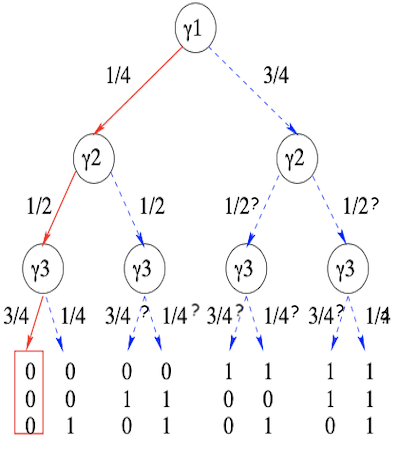
\includegraphics[keepaspectratio]{img/tree_v1.png}}

\section{Compositional Regression}\label{compositional-regression}

Approximate model \[\g \sim \N(\mub, \Sigmab_{\g})\]

\begin{itemize}
\item
  Wermouth (1980) compositional regression
  \[ \Gbf = \one_{T} \mub^T + (\G - \one_T \mub^T) \B + \eps
  \]
\item
  \(\Gbf\) is \(T \times p\) matrix where row \(t\) is \(\g_t\)
\item
  \(\mub\) is the \(p\) dimensional vector of \(\E[\g]\)
\item
  \(\Sigmab_{\g} = \U^T \U\) where \(\U\) is upper triangular Cholesky
  decomposition of covariance matrix of \(\g\) (\(p \times p\))
\item
  \(\B^T = \I_p -  diag(\U)^{-1} \U^{-T}\) (lower triangle)
\item
  \(\B\) is a \(p \times p\) upper triangular matrix with zeros on the
  diagonal and regression coefficients for \(jth\) regression in row
  \(j\)
\end{itemize}

\section{\texorpdfstring{Estimators of \(\B\) and
\(\mub\)}{Estimators of \textbackslash B and \textbackslash mub}}\label{estimators-of-b-and-mub}

\begin{itemize}
\item
  OLS is BLUE and consistent, but \(\Gbf\) may not be full rank
\item
  apply Bayesian Shrinkage with ``priors'' on \(\mub\) (non-informative
  or Normal) and \(\Sigma\) (inverse-Wishart)
\item
  pseudo-posterior mean \(\mub\) is the current estimate of the marginal
  inclusion probabilities \(\bar{\g} = \hat{\mub}\)
\item
  use pseudo-posterior mean for \(\Sigmab\)
\item
  one Cholesky decomposition provides all coefficients for the \(p\)
  predictions for proposing \(\g^*\)
\item
  constrain predicted values
  \(\hat{\rho}_{j \mid <j} \in (\delta, 1-\delta)\)
\item
  generate \(\g^*_j \mid \g^*_{< j} \sim \Ber(\hat{\rho}_{j \mid <j})\)
\item
  use as proposal for Adaptive Independent Metropolis-Hastings or
  Importance Sampling (Accept all) -or- Samping Without Replacement
  (todo)
\end{itemize}

\section{Simulation}\label{simulation}

\begin{itemize}
\item
  \texttt{tecator} data (Griffin et al (2021))
\item
  a sample of \(p = 20\) variables
\item
  compare

  \begin{itemize}
  \tightlist
  \item
    enumeration to
  \item
    MCMC with add, delete, and swap moves with \(q\)
  \item
    Adaptive Independent MCMC
  \item
    Importance Sampling with HT
  \end{itemize}
\item
  same settings \texttt{burnin.it}, \texttt{MCMC.it}, \texttt{thin}\\
\end{itemize}

\begin{Shaded}
\begin{Highlighting}[]
\FunctionTok{load}\NormalTok{(}\StringTok{"sim\_code/tecator{-}time.dat"}\NormalTok{)}
\FunctionTok{boxplot}\NormalTok{(time, }\AttributeTok{main=}\StringTok{"CPU time"}\NormalTok{, }\AttributeTok{ylab =} \StringTok{"Time"}\NormalTok{)}
\end{Highlighting}
\end{Shaded}

\pandocbounded{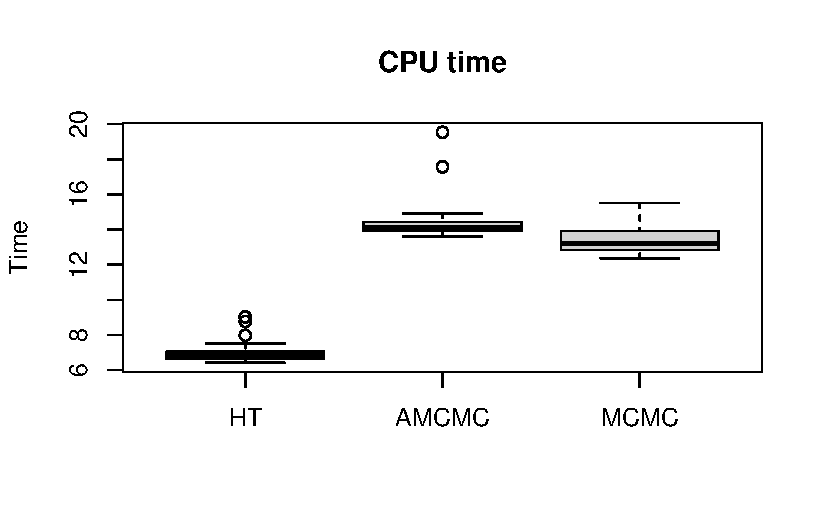
\includegraphics[keepaspectratio]{BMSSII-paper_files/figure-pdf/unnamed-chunk-2-1.pdf}}

\section{MSE Comparision}\label{mse-comparision}

\pandocbounded{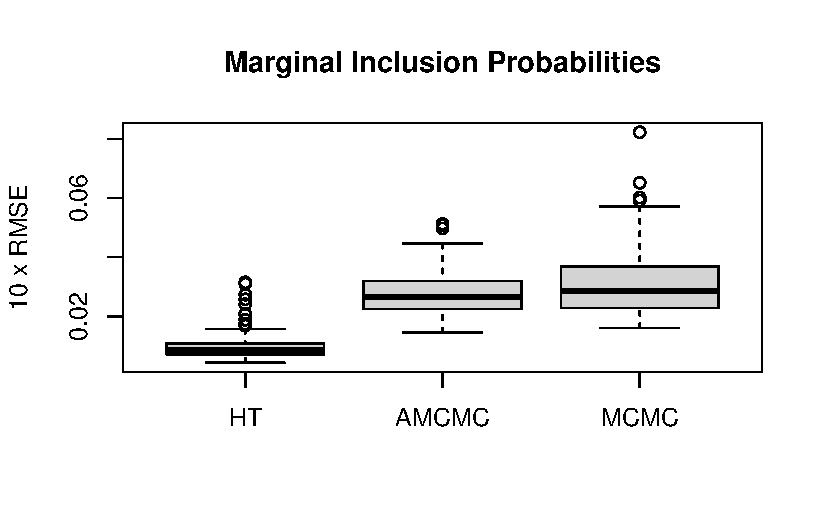
\includegraphics[keepaspectratio]{BMSSII-paper_files/figure-pdf/unnamed-chunk-3-1.pdf}}

\pandocbounded{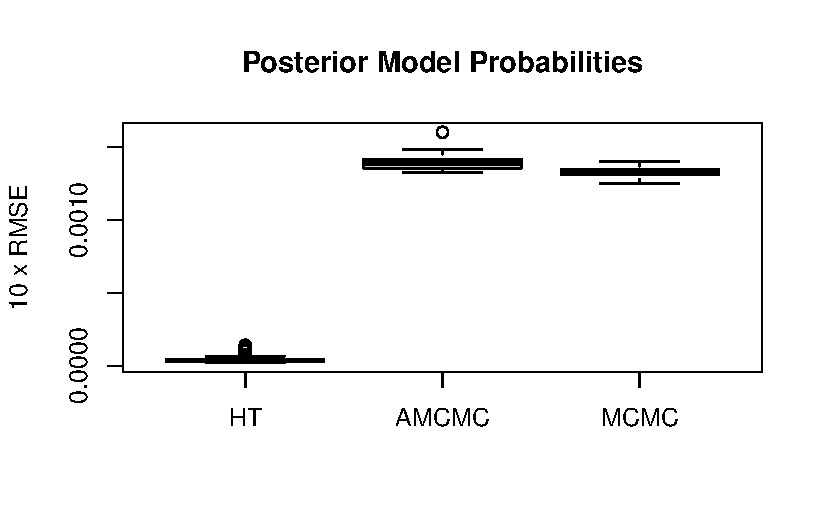
\includegraphics[keepaspectratio]{BMSSII-paper_files/figure-pdf/unnamed-chunk-4-1.pdf}}

\section{Continued Adaptation ?}\label{continued-adaptation}

\begin{itemize}
\tightlist
\item
  can update Cholesky with rank 1 updates with new models
\item
  how to combine IS with MH samples (weighting) ?
\item
  HT/Hajek - computational complexity involved if we need to compute
  inclusion probability for all models based on updates (previous models
  and future models)
\item
  Basu (1971) approach works with PPS-WOR take
  \(\pi_i \propto A_i \equiv q(\g_i)\) (adaptation?)
\end{itemize}

\section{Refinements}\label{refinements}

\begin{itemize}
\item
  Want to avoid MCMC for

  \begin{itemize}
  \tightlist
  \item
    pseudo Bayesian posteriors used to learn proposal distribution in
    sample design for models
  \item
    estimation of posterior model probabilities in model-based
    approaches (ie learning \(\beta\), sampling from predictive
    distribution)
  \item
    estimation of general quantities under BMA?
  \end{itemize}
\item
  avoid infinite regret
\item
  more general models?
\end{itemize}

\section{Summary}\label{summary}

\begin{itemize}
\tightlist
\item
  Adaptive Independent Metropolis proposal for models (use in more
  complex IS)
\item
  Use observed values of unique marginal likelihoods of models for
  estimating posterior distribution
\item
  Bayes estimates from MC output (solution to O'Hagan '73?)
\end{itemize}

::: ::::




\end{document}
